\section{Complex Numbers and Elementary Functions}
    \subsection{Properties}
    We define an imaginary number as
    \begin{align*} i^2 = -1 \end{align*}
    While a complex number is defined as
    \begin{align*} z = x + iy \end{align*}
    The common functions $\Re$ and $\Im$ yield the real and imaginary parts
    of a complex number respectively.\footnote{Also denoted as Re and Im} We
    can also express complex numbers in polar coordinates.
    \begin{align*}
        x &= r \cos \theta\\
        y &= r \sin \theta
    \end{align*}
    Using Euler's Identity,
    \begin{align*}
        \cos \theta + i \sin \theta = e^{i\theta}
    \end{align*}
    the alternate form is defined as
    \begin{align*}
        z &= x + iy = r \left(\cos \theta + i \sin \theta\right) = r e^{i\theta}\\
        r &= \sqrt{x^2 + y^2} = \abs{z}\\
        \tan \theta &= \frac{y}{x}
    \end{align*}
    The complex conjugate is defined as
    \begin{align*}
        x - iy \equiv r e^{-i\theta}
    \end{align*}
    We can define some common equivalences.
    \begin{easylist}[itemize]
        @ $\exp{\left(2\pi i \right)} = 1$
        @ $\exp{\left(\pi i\right)} = -1$
        @ $\exp{\left(\frac{\pi i}{2}\right)} = i$
        @ $\exp{\left(\frac{3\pi i}{2}\right)} = -i$
        @ $\exp{\left(i\theta_1\right)}\exp{\left(i\theta_2\right)} =
        \exp{\left(i\left(\theta_1 + \theta_2\right)\right)}$
        @ $\exp{\left(i\theta\right)}^m = \exp\left(im\theta\right)$
        @ $\exp{\left(i\theta\right)}^{1/n} =
        \exp\left(\frac{i\theta}{n}\right)$
    \end{easylist}

    Another neat trick is to let $z = 1/t$ to analyze behavior at $\infty$.

    \subsection{Stereographic Projection}
    We can visualize complex numbers with a stereographic projection. Zero
    is located at the North Pole, and infinity at the South Pole.
    \begin{figure}[H]
        \centering
        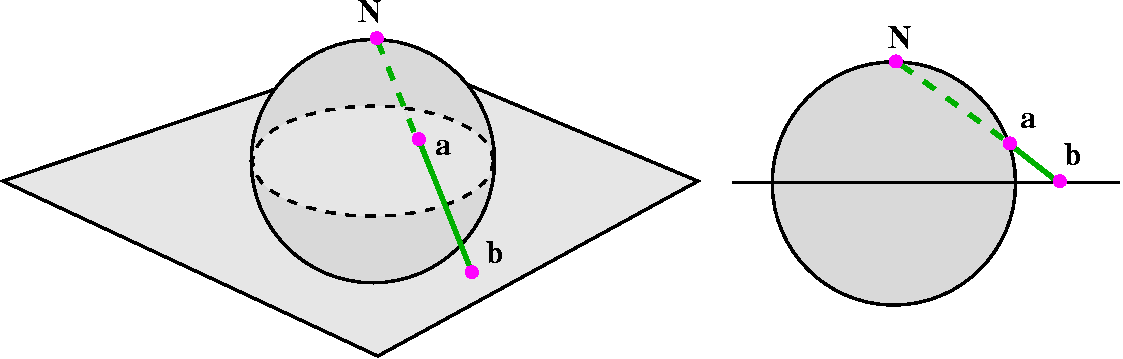
\includegraphics[scale=0.25]{./img/stereo.png}
        \caption{Stereographic Projection}
    \end{figure}
    These points are
    \begin{align*}
        X = \frac{4x}{\abs{z}^2 + 4} \qquad
        Y = \frac{4y}{\abs{z}^2 + 4} \qquad
        Z = \frac{2 \abs{z}^2}{\abs{z}^2 + 4}
    \end{align*}

    \subsection{Elementary Functions}
    Similar to Real Analysis, we can define a neighborhood of some point $z$ as
    the region enclosed by
    \begin{align*}
        \abs{z - z_0} < \epsilon
    \end{align*}
    As with sets, these can be closed, bounded, regions, domains, etc\ldots.

    We can also define functions of complex numbers, and as with real valued
    numbers, they mostly work the same. The simplest function is the power
    function.
    \begin{align*}
        f(z) = z^n
    \end{align*}
    Which can be extended to define Polynomials and rational functions (as
    the result of dividing a polynomial function with another).

    Limits also work the same, even with Radii of Convergence, etc.

    Projections and Mappings work intuitively.

    \subsection{Example - Rootfinding}
    Solve for all roots of the following equation: $z^4 + 2z = 0$.

    $z\pren{z^3 + 2} = 0$, so $z=0$ or $z^3 = -2$, and then $r^3=2$,
    $e^{3i\theta}=e^{i\pi}\Rightarrow\theta=\pi/3 + 2\pi n / 3$, $n=0, 1,
    2.$ Thus, the roots are
    \begin{align*}
        z = 0, 2^{1/3} e^{i \pi / 3}, 2^{1/3}e^{i \pi} = -2^{1/3},
        2^{1/3}e^{5i\pi / 3}
    \end{align*}

    \subsection{Limits}

    \begin{thm}[$\epsilon-\delta$ Limit Definition]
        A complex limit can be defined as
        \begin{align*}
            \lim_{z\to z_0} f(z) = w_0
        \end{align*}
        if for every sufficiently small $\epsilon > 0$, there is a $\delta > 0$
        such that
        \begin{align*}
            \abs{f(z) - w_0} < \epsilon \qquad \abs{z - z_0} < \delta
        \end{align*}
        This is the traditional $\epsilon-\delta$ format that we're used to from
        real analysis.
    \end{thm}

    Similarly, a function is said to be continuous if for all $z$,
    \begin{align*}
        \lim_{z\to z_0} f(z) = z_0
    \end{align*}
    The traditional definitions of Uniform and Absolute convergence also apply.

    Using these limit definitions we can define the concept of a derivative.
    \begin{align*}
        f^\prime (z_0) = \lim_{\Delta z \to 0}
            \pren{\frac{f(z_0 + \Delta z) - f(z_0)}{\Delta z}} =
        \lim_{z \to z_0}
            \pren{\frac{f(z) - f(z_0)}{z-z_0}}
    \end{align*}

    \subsection{Visualization}
    Is tricky. Wrote some code to rotate a complex function with static
    output supported. The hard part is you basically have a four-dimensional
    surface, since you have two input variables, the real and imaginary
    parts, and two output variables, the real and imaginary parts. The most
    straightforward way to visualize is to graph the output real and
    imaginary parts separately.
    \begin{figure}[H]
        \centering
        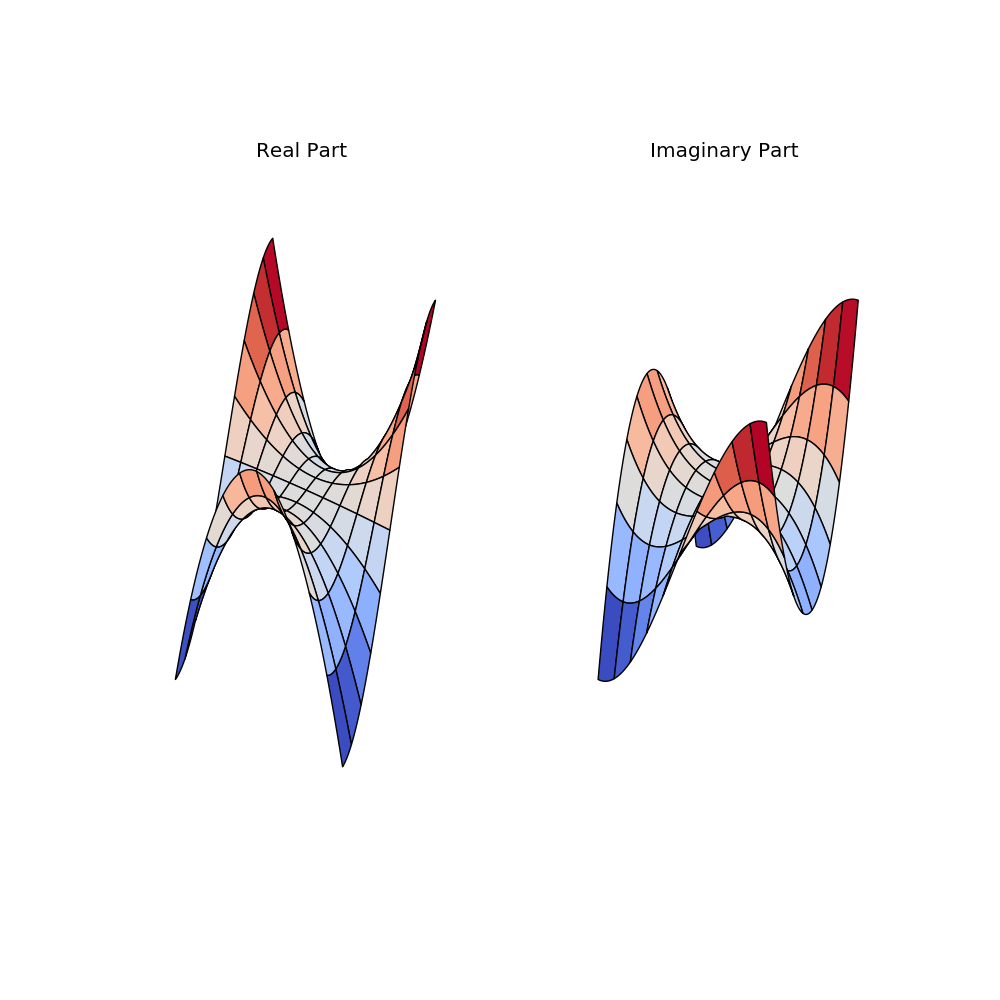
\includegraphics[scale=0.3]{./img/examplevis.png}
        \caption{Visualization of $f(z)=z^3$}
    \end{figure}

\section{Analytic Functions and Integration}

    \subsection{Analytic Functions}
    In order for a complex function to be differentiable, it has to satisfy
    the Cauchy-Riemann Conditions.
    \begin{thm}[Cauchy-Riemann Conditions]
        By writing the real and imaginary parts separately in the definition
        of a derivative, we get
        \begin{align*}
            f(z) &= u(x, y) + i v(x, y)\\
        f^\prime(z) &= \lim_{\Delta x \to 0} \pren{
            \frac{u(x + \Delta x, y) - u(x, y)}{\Delta x} +
            i \frac{v(x + \Delta x, y) - v(x, y)}{\Delta x}
        }\\
        &= u_x(x, y) + i v_x(x, y)
        \end{align*}
        Yielding the Cauchy-Riemann conditions,
        \begin{align*}
            u_x = v_y \qquad v_x = - u_y\\
            u_r = \frac{v_\theta}{r} \qquad v_r = -\frac{u_\theta}{r}
        \end{align*}
    \end{thm}

    \begin{thm}
        The function $f(z) = u(x, y) + i v(x, y)$ is differentiable at a
        point $z = x + iy$ of a region in the complex plane if and only if
        the partial derivatives $u_x$, $u_y$, $v_x$, $v_y$, are continuous
        and satisfy the Cauchy-Riemann conditions at $z=x+iy$.
    \end{thm}

    For differentiability, we can use the term analyticity to mean the same
    thing, both for pointwise differentiability and differentiability over a
    region. Points that are not differentiable (analytic) are called
    singular points.\footnote{Holomorphic is sometimes used as well (or
    instead) of analytic.}

    Some properties
    follow.\footnote{\url{https://en.wikipedia.org/wiki/Analytic_function\#Properties_of_analytic_functions}}
    \begin{easylist}[itemize]
        @ Sums, Products, and Compositions of analytic functions are
        analytic.
        @ The reciprocal of an analytic function that is nowhere zero is
        analytic, as is the inverse of an invertible analytic function whose
        derivative is nowhere zero.
    \end{easylist}

    An entire function is one that's analytic on the entire finite plane.

    Taking the second derivative of the Cauchy-Riemann conditions yields
    Laplace's Equation.
    \begin{align*}
        u_{xx} = v_{xy} \qquad v_{yx} = -u_{yy}\\
        \nabla^2 w = 0 \Rightarrow \begin{cases}
            \nabla^2 u \equiv u_{xx} + u_{yy} = 0\\
            \nabla^2 v \equiv v_{xx} + v_{yy} = 0
        \end{cases}
    \end{align*}
    A function that satisfies the concise Laplace Equation: $\nabla^2 w = 0$
    is called a harmonic function in D. $u$ and $v$ are referred to as
    harmonic functions in D, and they are harmonic conjugates of each other.

    \subsection{Example - Cauchy-Riemann Conditions}
    Let $f(z) = e^z = e^{x+i y} = e^x e^{iy} = e^x \pren{\cos y + i \sin
    y}$. Verify Cauchy-Riemann for all $x$, $y$, and then show that
    $f^\prime(z) = e^z$.
    \begin{align*}
        u = e^x \cos y \qquad v = e^x \sin y\\
        u_x = e^x \cos y = v_y\\
        v_y = -e^x \sin y = -v_x\\
        f^\prime(z) = u_x + i v_x = e^x \pren{\cos y + i \sin y} = e^z
    \end{align*}

    \subsection{Ideal Fluid Flow - Application of Laplace's Equation}
    Two dimensional ideal fluid flow is a great example of Laplace's
    Equation. This is fluid that is time independent, nonviscous,
    incompressible, and irrotational.
    \begin{easylist}[enumerate]
        @ Incompressibility:
        \begin{align*}
            v_{1,x} + v_{2, y} = 0
        \end{align*}
        Where $v_1$ and $v_2$ are the horizontal and vertical components.
        @ Irrotationality:
        \begin{align*}
            v_{2, x} - v_{1, y} = 0
        \end{align*}
        @ Simplified:
        \begin{align*}
            v_1 = \phi_x = \psi_y \qquad v_2 = \phi_y = -\psi_x\\
            \vec{v} = \nabla \phi
        \end{align*}
        $\phi$ is the velocity potential, and $\psi$ the stream function.
        Cauchy-Riemann is satisfied for $\phi$ and $\psi$, therefore we have
        a complex velocity potential.
        \begin{align*}
            \Omega(z) &= \phi(x, y) + i \psi(x, y)\\
            \Omega^\prime(z) &= \phi_x + i \psi_x =
            \phi_x - i \psi_y =
            v_1 - v_2
        \end{align*}
    \end{easylist}

    \subsection{Example - Uniform Flow}
    Uniform Flow is
    \begin{align*}
        \Omega(z) = v_0 e^{-i \theta_0} z =
        v_0 \pren{\cos \theta_0 - i \sin \theta_0}\pren{x + i y}
    \end{align*}
    where $v_0$ and $\theta_0$ are positive real constants. The
    corresponding velocity potential and velocity field is given by
    \begin{align*}
        \phi(x,y)=v_0\pren{\cos\pren{\theta_0 x}+\sin\pren{\theta_0 y}}\\
        v_1 = \phi_x = v_0 \cos \theta_0 \qquad
        v_2 = \phi_y = v_0 \sin \theta_0
    \end{align*}
    which is identified with uniform flow making an angle $\theta_0$ with
    the $x$ axis. Alternatively, the steam function $\psi(x, y) = v_0
    \pren{\cos\pren{\theta_0 y} - \sin\pren{\theta_0 x}} = \text{const.}$
    reveals the same flow field.

    \subsection{Multivalued Functions}
    A simple example of this is the square root function which takes on
    different values for $n$ even or odd.
    \begin{align*}
        z = w^2 \qquad w &= \sqrt{z}\\
        &= r^{1/2}e^{i\theta_p / 2}e^{n \pi i}
    \end{align*}
    We can define these ``points'' where complex functions take on multiple
    values as branch points. In the same way that they're referred to as
    branch points, branches of a multivalued function are when we restrict
    to only one set of continuous values. A branch cut is this restriction
    process.\footnote{The real analogy here is a function like $\pm\sqrt{x},
        x\in\mathbb{R}$.  $0$ is a branch point, and we often times just
        examine the branch where $\sqrt{x} > 0$. The analogous branch cut is
    $x > 0$.}

    Log is more complicated, and we define it as such.
    \begin{align*}
        w = \log(z) = \log r + i \theta_p + 2n\pi i,
        \qquad n = 0, \pm 1, \pm 2, \ldots,
        \qquad 0 \le \theta_p < 2\pi
    \end{align*}

    \subsection{Example - Branch Points/Cuts}
    Find the location of the branch points and discuss possible branch cuts
    for the following functions:
    \begin{easylist}[enumerate]
        @ $\pren{z - i}^{1/3}$

        Let $z - i = \epsilon e^{i \theta_p}$ which is a circular contour
        centered at $z = i$. We have just a power function in terms of
        $\zeta=z-i$, so $z=i$ and $z=\infty$ are branch points. Any line
        connecting $z = \infty$ and $z=i$ is a branch cut, e.g.\
        $\cren{z=iy|y\in[1,+\infty)}$ is as good as any. There are 3
        distinct branches.

        @ $\log\pren{\frac{1}{z-2}}$

        $\log\pren{\frac{1}{z-2}} = -\log\pren{z-2}$. Again, this is
        $-\log(z)$ but with shiftd origin. So the branch points are $z=2$
        and $z=\infty$. A branch cut must connect the branch points, it can
        be $\cren{z=x|x\in[2,+\infty)}$ or $\cren{z=x|x\in(-\infty,2]}$.
    \end{easylist}

    \subsection{Example - Rootfinding (cont.)}
    Solve for all values of $z$: $4 + 2e^{z + i} = 2$.
    \begin{align*}
        4 + 2e^{z + i} = 2 \Rightarrow
        e^{z+i} = -1 = e^{i\pi + 2\pi i n}, n \in \mathbb{Z}
    \end{align*}
    Therefore
    \begin{align*}
        z+i = i \pi + 2 \pi i n \Rightarrow
        z = i\pren{\pi - 1 + 2 \pi n}, n \in \mathbb{Z}
    \end{align*}

    \subsection{Example - Branch Points/Cuts (cont.)}
    Find the location of the branch points and discuss a branch cut
    structure associated with the function:
    \begin{easylist}[itemize]
        @ $f(z) = \frac{z - 1}{z}$

        This is a rational function singular at $z=0$, but single-valued, so
        no branch points.

        @ $f(z) = \log\pren{z^2 - 3}$

        Here $z^2 - 3$ is entire single-valued function so the only branch
        points are those where $z^2 - 3 = 0$ or $z^2 - 3 = \infty$. Thus,
        there are three branch points, $z=\pm\sqrt{3}$, and $z=\infty$. A
        branch cut must make sure there is no possibility going around and
        single of them, in this case it must connect all three points. E.g.\
        consider a cut on real axis $\cren{z=x|x\in[-3,+\infty)}$.

        @ $f(z) = \exp{\sqrt{z^2 - 1}}$

        Since function $e^z$ is entire (analytic on plane) the only possible
        branch points are those of $\sqrt{z^2-1}$, i.e.\ $z = \pm 1$ and
        $z=\infty$. However, doing the circle argument
        $z-1=r_1e^{i\theta_1}$, $z+1=r_2e^{i\theta_2}$,
        $\theta_1\to\theta_1+2\pi$, $\theta_2\to\theta_2+2\pi$, one sees
        that $z=\infty$ is not a branch point since $\exp{\pren{2\pi i + 2
        \pi i} / 2} = 1$ which corresponds to encircling both $z=1$ and
        $z=-1$, equivalent to encircling just $z=\infty$. Thus, $z=\infty$
        is not a branch point even for $\sqrt{z^2 - 1}$. But $z=\pm 1$ are
        branch points, and a branch cut connecting them is
        $\cren{z=x|x\in[-1,1]}$.
    \end{easylist}

    \subsection{More Complicated Multivalued Functions and Riemann
    Surfaces}
    If we have functions like the following
    \begin{align*}
        w = \bren{\pren{z-a}\pren{z-b}}^{1/2}
    \end{align*}
    We need to use a slightly more complicated branch cut/structure. We know
    that the points $z=a, b$ are both branch points (by letting
        $z=a+\epsilon_1 e^{i\theta_1}$ and as $\theta_1$ varies from $0$ to
    $2\pi$, $w$ jumps from $q^{1/2}$ to $-q^{1/2}$), and so we can define a
    branch cut as follows.
    \begin{align*}
        z-b&=r_1e^{i\theta_1}\\
        z-a&=r_2e^{i\theta_2} \qquad 0 \le \theta_1, \theta_2 < 2 \pi
    \end{align*}
    Our equation now becomes
    \begin{align*}
        w=\pren{r_1r_2}^{1/2} e^{i\pren{\theta_1 + \theta_2} / 2}
    \end{align*}
    This process extends to more complicated functions, as for any $w$ of
    the form
    \begin{align*}
        w=\bren{\pren{z-x_1}\pren{z-x_2}\cdots\pren{z-x_n}}^{m}
    \end{align*}
    we can define our branch cuts to be
    \begin{align*}
        z - x_k = r_k e^{i\theta_k}
    \end{align*}
    yielding
    \begin{align*}
        w=\pren{r_1r_2\cdots r_n}
        e^{m i \pren{\theta_1 + \theta_2 + \cdots + \theta_n}}
    \end{align*}

    \subsection{Example - Branch Points/Cuts (cont.)}
    Find the location of branch points and discuss a branch cut structure
    associated with the function:
    \begin{align*}
        f(z) = \coth^{-1} \frac{z}{a} = \frac{1}{2}
        \log\pren{\frac{z+a}{z-a}}, a > 0
    \end{align*}
    This is (up to a constant) log of rational function, so the branch
    points are those where $\pren{z+a} / \pren{z-a} = 0$ or $\infty$, i.e.\
    $z=\pm a$. As for $z=\infty$, it is not a branch point, as the limit
    equals 1, not zero. A cut must connect the two points, so a possible one
    is interval $[-a,a]$ on the real axis.

    \subsection{Riemann Surfaces}
    Instead of considering the normal complex plane with arbitrary ``cuts'',
    it can be useful to instead consider a surface with multiple ``sheets''.
    Any multivalued function only has one point that corresponds to each
    point on the sheet. This way, for any given sheet, the function is
    single-valued.

    For the function $w^{1/2}$, since we have two branches, our Riemann
    surface is two-sheeted. For the log function, since it is infinitely
    multivalued, we have infinite sheets.

    \begin{figure}[H]
        \centering
        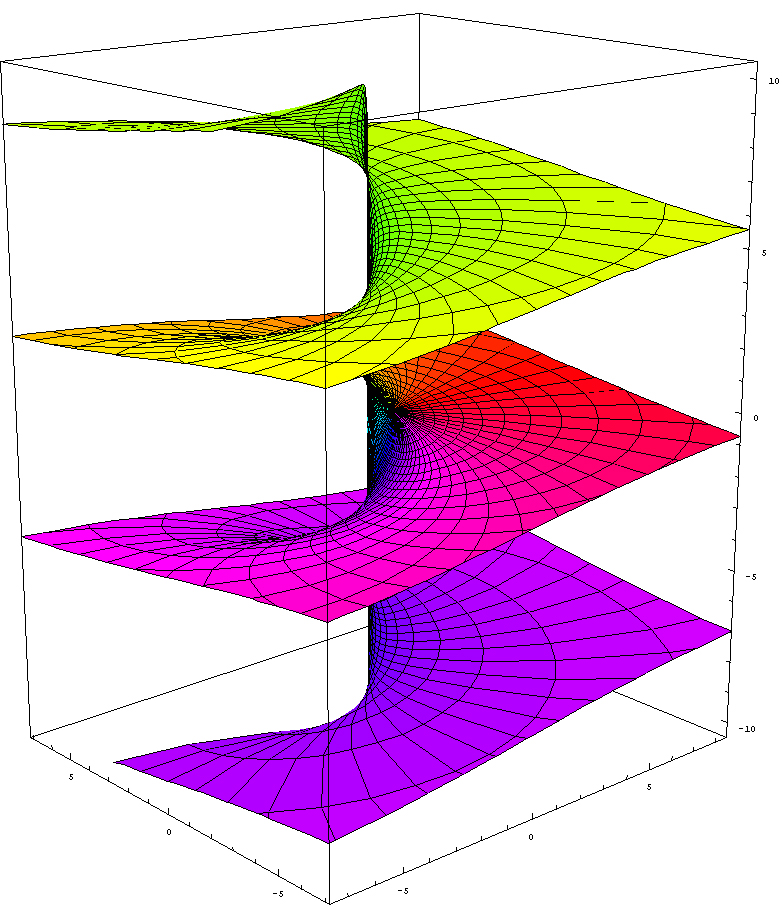
\includegraphics[scale=0.3]{./img/Riemann_surface_log.png}
        \caption{Riemann Surface for $\log(z)$}
    \end{figure}

    \subsection{Complex Integration}
    Consider a function $f(t) = u(t) + i v(t)$. This function is integrable
    if $u$ and $v$ are integrable (with the same properties applying).
    \begin{align*}
        \int_a^b f(t) \, dt = \int_a^b u(t) \, dt + i \int_a^b v(t) \, dt
    \end{align*}
    Defining a curve on the complex plane can be done parametrically, with
    form\footnote{These curves are
        \begin{itemize}
            \item \textbf{Simple Curve} or \textbf{Jordan Arc} if it does not
            intersect itself.
            \item \textbf{Simple Closed Curve} or \textbf{Jordan Curve} if the
            endpoints meet.
        \end{itemize}}
    \begin{align*}
        z(t) = x(t) + i y(t)
    \end{align*}
    The path (contour) integral of function $f$ on contour $z$ is defined to
    be\footnote{Contours are defined as piecewise smooth connected arcs.
    Simple closed is referred to as a Jordan Contour}
    \begin{align*}
        \int_C f(z) \, dz = \int_a^b f(z(t))z^\prime(t) \, dt
    \end{align*}
    This is really a line integral in the $(x, y)$ plane.

    \begin{thm}
        Suppose $F(z)$ is an analytic function and that $f(z) = F^\prime(z)$
        is continuous in a domain $D$. Then for a contour $C$ lying in $D$
        with endpoints $z_1$ and $z_2$
        \begin{align*}
            \int_C f(z) \, dz = F(z_2) - F(z_1)
        \end{align*}
        Since we can think of the parameterized complex plane as a vector
        field, for closed curves, we have
        \begin{align*}
            \oint_C f(z) \, dz = \oint_C F^\prime(z) \, dz = 0
        \end{align*}
        Note that everything here hinges on the analyticity of $F$ and the
        continuity in domain $D$.
    \end{thm}

    \begin{thm}
        Let $f(z)$ be continuous on a contour $C$. Then
        \begin{align*}
            \abs{\int_C f(z) \, dz} \le ML
        \end{align*}
        where $L$ is the length of $C$ and $M$ is an upper bound for
        $\abs{f}$ on $C$.

        Arc length can be defined (from Calc III) for a parameterized curve
        with form $z(t) = u(t) + i v(t)$ as
        \begin{align*}
            \int_a^b \sqrt{\pren{u^\prime(t)}^2 + \pren{v^\prime(t)}^2} \, dt
        \end{align*}
    \end{thm}

    Hey, this is nice and easy! If the given function is analytic on and in
    its domain, then it just equals zero! If there is a singularity on the
    inside of the domain, deform the contour so that you have 2 curves of
    opposite direction. Then $C_1 = C_2$, and you can just solve for the one
    that surrounds the singularity.

    \subsection{Example - Contour Integration}
    Evaluate $\int_C \overline{z} \, dz$ for a contour from $z=0$ to $z=1$
    to $z=1+i$.
    \begin{align*}
        \int_C\overline{z}\,dz &= \int_C \pren{x - iy}\pren{dx + i \, dy}\\
        &= \int_{x=0}^1 x \, dx + \int_{y=0}^1 \pren{1 - iy}\pren{i \, dy}\\
        &= \frac{1}{2} + i \bren{y - iy^2 / 2}^1_0\\
        &= 1 + i
    \end{align*}

    \subsection{Cauchy's Theorem}

    \begin{thm}[Cauchy]
        If a function $f$ is analytic in a simply connected domain $D$, then
        along a simple closed contour $C$ in $D$
        \begin{align*}
            \oint_C f(z) \, dz = 0
        \end{align*}
        We also require that $f^\prime(z)$ is also continuous in $D$.

        ``If $f(z)$ is analytic everwhere interior to and on a simple closed
        contour $C$, then $\oint_C f(z) \, dz = 0$.''

        Again, NOTE that everything hinges on the fact that $D$ must be
        simply connected. In order to use this, you need a simply connected
        domain $D$ AND a simple closed contour $C$.
    \end{thm}

    To best apply Cauchy's Theorem, we can use tricks like turning a complex
    contour into several simple contours, and deforming a simply connected
    domain so that the function is analytic on the domain.

    \subsection{Example - Cauchy's Theorem}
    Evaluate
    \begin{align*}
        \mathcal{I} = \frac{1}{2\pi i} \oint_C \frac{1}{\pren{z-a}^m} \, dz
        , \qquad m = 1, 2, \ldots, M
    \end{align*}
    where $C$ is a simple closed contour.

    The function $f(z) = 1 / \pren{z-a}^m$ is analytic for all $z \neq a$.
    Hence if $C$ does not enclose $z=a$, then we have $\mathcal{I}=0$. If
    $C$ encloses $z=a$, we use Cauchy's Theorem to deform the contour to
    $C_a$, a small, but finite circle of radius $r$ centered at $z=a$.
    Namely,
    \begin{align*}
        \int_C f(z) \, dz - \int_{C_a} f(z) \, dz = 0, \qquad f(z) = 1 / \pren{z-a}^m
    \end{align*}
    We evaluate $\int_{C_a} f(z) \, dz$ by letting
    \begin{align*}
        z - a = r e^{i \theta}, \qquad dz = i e^{i\theta} r d\theta
    \end{align*}
    in which case
    \begin{align*}
        \mathcal{I} &= \frac{1}{2\pi i} \oint_C \frac{1}{\pren{z-a}^m} \, dz
        = \frac{1}{2\pi i} \int_0^{2\pi} \frac{1}{r^m e^{im\theta}} i
        e^{i\theta} r \, d\theta\\
        &= \frac{1}{2\pi i} \int_0^{2\pi} i
        e^{-i\pren{m-1}\theta}r^{-m+1}\,d\theta = \delta_{m,1} =
        \begin{cases}
            1 \quad m = 1\\
            0 \quad \text{else}
        \end{cases}
    \end{align*}
    Therefore,
    \begin{align*}
        \mathcal{I}=\begin{cases}
            0 \quad z = a \text{ outside } C\\
            0 \quad z = a \text{ inside } C, \quad m \neq 1\\
            1 \quad z = a \text{ inside } C, \quad m = 1
        \end{cases}
    \end{align*}

    \subsection{Example - Polynomials and Cauchy's Theorem}
    Let $P(z)$ be a polynomial of degree $n$, with $n$ simple roots, none of
    which lie on a simple clsoed contour $C$. Evaluate
    \begin{align*}
        \mathcal{I}=\frac{1}{2\pi i} \oint_C \frac{P^\prime(z)}{P(z)} \, dz
    \end{align*}
    Because $P(z)$ is apolynomial with distinct roots, we can factor it as
    \begin{align*}
        P(z)=A\pren{z-a_1}\pren{z-a_2}\cdots\pren{z-a_n}
    \end{align*}
    Where $A$ is the coefficient of the term of highest degree. Because
    \begin{align*}
        \frac{P^\prime(z)}{P(z)} &= \frac{d}{dz} \pren{\log P(z)}
        &= \frac{d}{dz} \log \pren{A\pren{z-a_1}\pren{z-a_2}\cdots\pren{z-a_n}}
    \end{align*}
    it follows that
    \begin{align*}
        \frac{P^\prime(z)}{P(z)} &= \frac{1}{z-a_1} +\frac{1}{z-a_2} +
        \cdots + \frac{1}{z-a_1}
    \end{align*}
    Hence, using the same method as above, we have
    \begin{align*}
        \mathcal{I}=\frac{1}{2\pi i} \oint_C \frac{P^\prime(z)}{P(z)} \, dz
        = \text{number of roots lying within } C
    \end{align*}

    \subsection{Cauchy's Integral Formula, Its $\overline{\partial}$
    Generalization and Consequences}

    \begin{thm}
        Let $f(z)$ be analytic interior to and on a simple closed contour
        $C$. Then at any interior point $z$
        \begin{align*}
            f(z) = \frac{1}{2\pi i}
            \oint_C \frac{f(\zeta)}{\zeta - z} \, d\zeta
        \end{align*}
        This is referred to as Cauchy's Integral Formula.
    \end{thm}

    \begin{thm}
        If $f(z)$ is analytic interior to and on a simple closed contour $C$
        then all the derivatives $f^{(k)}(z),k=1,2,\ldots$ exist in the
        domain $D$ interior to $C$, and
        \begin{align*}
            f^{(k)}(z) = \frac{k!}{2 \pi i}
            \oint_C \frac{f(\zeta)}{\pren{\zeta - z}^{k+1}} \, d\zeta
        \end{align*}
    \end{thm}

    \begin{thm}
        All partial derivatives of $u$ and $v$ are continuous at any point
        where $f=u+iv$ is analytic.
    \end{thm}

    \begin{thm}[Lioville]
        If $f(z)$ is entire and bounded in the $z$ plane (including
        infinity), then $f(z)$ is a constant.
    \end{thm}

    \begin{thm}[Morera]
        If $f(z)$ is continuous in a domain $D$ and if
        \begin{align*}
            \oint_C f(z) \, dz = 0
        \end{align*}
        for every simple closed contour $C$ lying in $D$, then $f(z)$ is
        analytic in $D$.
    \end{thm}

    \begin{thm}[Maximum Principles]
        \begin{easylist}[enumerate]
            @ If $f(z)$ is analytic in a domain $D$, then $\abs{f(z)}$
            cannot have a maximum in $D$ unless $f(z)$ is a constant.
            @ If $f(z)$ is analytic in a bounded region $D$ and $\abs{f(z)}$
            is continuous in the closed region $\overline{D}$, then
            $\abs{f(z)}$ assumes its maximum on the boundary of the region.
        \end{easylist}
    \end{thm}

    \begin{thm}[Generalized Cauchy Formula]
        If $\partial f / \partial \overline{\zeta}$ exists and is continuous
        in a region $R$ bounded by a simple closed contour $C$, then at any
        interior point $z$
        \begin{align*}
            f(z) =
            \frac{1}{2 \pi i}
            \oint_C \pren{\frac{f(\zeta)}{\zeta - z}}\,d\zeta -
            \frac{1}{\pi}
            \iint_R \pren{\frac{\partial f / \partial
            \overline{\zeta}}{\zeta-z}}\,dA(\zeta)
        \end{align*}
    \end{thm}

    \subsection{Example - Cauchy's Theorem}
    Evaluate the integral $\oint_C f(z) \, dz$ where $C$ is the unit circle
    enclosing the origin and $f(z)$ is given by
    \begin{easylist}[itemize]
        @ $\log(z - z_0), z_0 > 1$

        Consider an analytic branch of $\log\pren{z-z_0}$ such that branch
        cut joining $z_0$ and $\infty$ does not cross the unit circle
        centered at $z=0$. Then $\log\pren{z-z_0}$ is analytic inside $C$
        and, by Cauchy's Theorem, $\oint_C \log\pren{z-z_0} \, dz = 0$.
        @ $z / \pren{z^2 + a^2}, \abs{a} < 1$

        \begin{align*}
            \frac{z}{z^2 + a^2} = \frac{1}{2 \pren{z-ia}} +
            \frac{1}{2\pren{z+ia}}
        \end{align*}
        $z=\pm ia$ are the singularities of $f(z)$ inside the contour. For
        each summand we find
        \begin{align*}
            \oint_C
            \frac{1}{2 \pren{z-ia}}
            \, dz = \pi i \qquad
            \oint_C
            \frac{1}{2\pren{z+ia}}
            \, dz = \pi i
        \end{align*}
        so $\oint_C f(z) dz = \pi i + \pi i = 2 \pi i$.
    \end{easylist}

    Evaluate the integral
    \begin{align*}
        \oint_C \pren{\frac{2e^{iz}}{z} + \frac{1}{z-\pi}} \, dz
    \end{align*}
    Where $C$ is
    \begin{easylist}[itemize]
        @ A boundary of the annulus between circles of radius 1 and radius 4
        with centers at the origin

        Use
        \begin{align*}
            \oint_C \pren{\frac{2e^{iz}}{z} + \frac{1}{z-\pi}} \, dz =
            \oint_C \frac{2e^{iz}}{z} \, dz +
            \oint_C \frac{1}{z-\pi} \, dz = I_1 + I_2
        \end{align*}
        and compute $I_1$ and $I_2$ separately.  For $I_1$, the integrated
        function is analytic everywhere except $z=0$ which is outside the
        annulus. Cutting the annulus and using Cauchy theorem for the cut
        annulus we find that $I_1 = 0$. Since $1<\pi<4$, the point $z=\pi$
        is inside the annulus and we find
        \begin{align*}
            I_2 =
            \oint_C \frac{1}{z-\pi} \, dz
            = 
            \oint_{\abs{z}=1} \frac{1}{z-\pi} \, dz
            +
            \oint_{\abs{z}=4} \frac{1}{z-\pi} \, dz
            = 0 + 2\pi i = 2\pi i
        \end{align*}
        Where we used Cauchy theorem for the first integral and deformation
        of the contour to a small circle with center $z=\pi$ for the second.
        Thus we obtain $I_1 + I_2 = 2\pi i$.

        @ A circle of radius $R$, $R>5$, with center at the origin.

        Here, since $\pi < 5$, we obtain $I_2 = 2\pi i$ like for the annulus
        above. As for $I_1$, we expand $e^{iz}$ in the Taylor series
        (converging for all $z$) and find
        \begin{align*}
            I_1 = \oint_C \frac{2e^{iz}}{z} \, dz = \oint_{\abs{z}=R}
            \frac{2}{z} \pren{1 + iz + \frac{\pren{iz}^2}{2} + \cdots} \, dz
            = \oint_{\abs{z}=R} \pren{\frac{2}{z} + 2i - z + \cdots} \, dz =
            4 \pi i + 0 = 4 \pi i
        \end{align*}
        where only the first term gives non-zero contribution. Thus
        $I_1+I_2=6\pi i$.
    \end{easylist}

    Evaluate the integral $\oint_C f(z) dz$ where $C$ is the unit circle
    centered at the origin for the following $f(z)$.

    The only singular point in both is $z=0$. We will expand the numerators
    in Taylor series around zero and use the integration of powers formula.
    \begin{easylist}[itemize]
        @ \begin{align*}
            \frac{e^{z^2}}{z} = \frac{1}{z} \sum_{n=0}^\infty
            \frac{z^2n}{n!} = \sum_{k=-1}^\infty \frac{z^{2k+1}}{\pren{k+1}!}
        \end{align*}
        power $z^{-1}$ corresponds to $k=-1$, thus $\oint_C f(z) \, dz =
        2\pi i$.
        @ \begin{align*}
            \frac{\sin z}{z^4} = \frac{1}{z^3} - \frac{1}{6z} +
            \frac{z}{120} + \cdots
        \end{align*}
        so $\oint_C f(z) \, dz = -2\pi i / 6 = -i \pi / 3$.
    \end{easylist}

    Let $f(z)$ be an entire function with $\abs{f(z)} \le C \abs{z}$ for all
    $z$, where $C$ is a constant. Show that $f(z) = Az$, where $A$ is a
    constant.

    Using the generalized Cauchy formula,
    \begin{align*}
        f^\prime(z) = \frac{1}{2\pi i} \oint_C
        \frac{f(\zeta)}{\pren{\zeta-z}^2} \, d\zeta
    \end{align*}
    where $C=\{\abs{\zeta - z} = R \}$ is the circle of radius $R$ around
    $z$ in the $\zeta$-plane. Then
    \begin{align*}
        \abs{f^\prime} \le \frac{1}{2\pi} \oint_C
        \frac{\abs{f(\zeta)}}{\abs{\zeta - z}^2} \, \abs{d\zeta} \le
        \frac{1}{2\pi} \int_0^{2\pi} \frac{C\pren{\abs{z} + R}}{R^2} R
        d\theta = C\pren{1+\abs{z}/R} = C
    \end{align*}
    So $f^\prime(z)$ is entire and bounded, so it is constant by Liouville
    theorem. Let $f^\prime(z) = A$, then $f(z)=Az+B$, where $A, B$ are
    constants. But, since $\abs{f(z)} \le C\abs{z}$ for all $z$, taking
    $\abs{z}\to0$, we get $B=0$. Thus, $f(z) = Az$ as claimed.

    \subsection{Theoretical Developments}
    \begin{thm}[Cauchy-Goursat]
        If a function $f(z)$ is analytic at all points interior  to and on a
        simple closed contour, then
        \begin{align*}
            \oint_C f(z) \, dz = 0
        \end{align*}
    \end{thm}

\section{Sequences, Series, and Singularities of Complex Functions}
    \subsection{Definitions of Complex Sequences, Series, and Their Basic
    Properties}
    We can denote a sequence of functions that converge to some given
    function as
    \begin{align*}
        \lim_{n\to\infty} f_n(z) = f(z) \Leftrightarrow
        \abs{f_n(z) - f(z)} < \epsilon
    \end{align*}

    If the limit does not exist, or is infinite, the sequence is said to
    diverge for those values of $z$.

    We say the sequence of functions converges uniformly if we can choose
    $N$ on only $\epsilon$, and not $z$. In other words, if for any $z$, the
    $n^{th}$ function is $\epsilon$ close to $f(z)$.

    \begin{thm}
        Let the sequence of functions $f_n(z)$ be continuous for each
        integer $n$ and let $f_n(z)$ converge to $f(z)$ uniformly in a
        region $\mathcal{R}$. Then $f(z)$ is continuous, and for any finite
        contour $C$ inside $\mathcal{R}$
        \begin{align*}
            \lim_{n\to\infty} \int_C f_n(z) \, dz = \int_C f(z) \, dz
        \end{align*}
    \end{thm}

    \begin{thm}[Weierstrass M Test]
        Let $\abs{b_j(z)} \le M_j$ in a region $\mathcal{R}$, with $M_j$
        constant. If $\sum_{j=1}^\infty M_j$ converges, then the series
        $S(z)=\sum_{j=1}^\infty b_j(z)$ converges uniformly in
        $\mathcal{R}$.
    \end{thm}

    \begin{thm}[Corollary: Ratio Test]
        Suppose $\abs{b_1(z)}$ is bounded, and
        \begin{align*}
            \abs{\frac{b_{j+1}(z)}{b_j(z)}} \le M < 1, \qquad j > 1
        \end{align*}
        for $M$ constant. Then the series
        \begin{align*}
            S(z) = \sum_{j=1}^\infty b_j(z)
        \end{align*}
        is uniformly convergent.
    \end{thm}
    \subsection{Example - Convergence}
    Show that the following series converges uniformly in the given region:
    $\sum_{n=1}^\infty z^n , 0 \le \abs{z} < R , R < 1$
    \begin{align*}
        \abs{\sum_{n=1}^\infty z^n} \le \sum_{n=1}^\infty \abs{z}^n
        \le \sum_{n=1}^\infty R^n = \frac{R}{1-R}
    \end{align*}
    i.e.\ the series is bounded above by a convergent numerical series,
    which means numerical convergence by the Weierstrass M-test.

    \subsection{Example - Radius of Convergence}
    \begin{easylist}[itemize]
        @ $z^{2n}$
        \begin{align*}
            z^{2n} = \pren{z^2}^n\\
            \abs{\frac{a_n}{a_{n+1}}}
            = \abs{\frac{z^{2n}}{z^{2\pren{n+1}}}}
            = \frac{1}{\abs{z}^2}
        \end{align*}
        Therefore it converges for $\abs{z} < 1$ and the radius of
        convergence is $R=1$.
        @ $n^n z^n$
        \begin{align*}
            \abs{\frac{a_n}{a_{n+1}}}
            = \abs{\frac{n^n z^n}{\pren{n+1}^\pren{n+1} z^{n+1}}}
            = \frac{1}{\pren{n+1}\pren{1 + 1/n}^n \abs{z}} = 0
        \end{align*}
        Therefore $R=0$.
    \end{easylist}
    \subsection{Taylor Series}
    A power series about the point $z=z_0$ is defined as
    \begin{align*}
        f(z) = \sum_{j=0}^\infty b_j \pren{z - z_0}^j\\
        f(z+z_0) = \sum_{j=0}^\infty b_j z^j
    \end{align*}
    With $b_j$, $z_0$ are constants. WLOG\footnote{Without Loss Of
    Generality} we can work with
    \begin{align*}
        f(z) = \sum_{j=0}^\infty b_j z^j
    \end{align*}
    which is the $z_0 = 0$ case.
    \begin{thm}
        If the series
        \begin{align*}
            f(z) = \sum_{j=0}^\infty b_j z^j
        \end{align*}
        converges for some $z_* \neq 0$, then it converges for all $z$ in
        $\abs{z} < \abs{Z_*}$. Morever, it converges uniformly in $\abs{z}
        \le R$ for $R < \abs{Z_*}$.
    \end{thm}
    \begin{thm}[Taylor Series]
        Let $f(z)$ be analytic for $\abs{z} \le R$. Then
        \begin{align*}
            f(z) = \sum_{j=0}^\infty b_j z^j
        \end{align*}
        where
        \begin{align*}
            b_j = \frac{f^{(j)}(0)}{j!}
        \end{align*}
        converges uniformly in $\abs{z} \le R_1 < R$.
    \end{thm}

    The largest number $R$ for which the power series converges inside the
    disk $\abs{z} < R$ is called the radius of convergence.

    \begin{thm}
        Let $f(z)$ be analytic for $\abs{z} \le R$. Then the series obtained
        by differentiating the Taylor series termwise converges uniformly to
        $f^\prime(z)$ in $\abs{z} \le R_1 < R$.
    \end{thm}

    \begin{thm}
        If the power series converges for $\abs{z} \le R$, then it can be
        differentiated termwise to obtain a uniformly convergent series for
        $\abs{z} \le R_1 < R$.
    \end{thm}

    \begin{thm}[Comparison Test]
        Let the series $\sum_{j=0}^\infty a_j z^j$ converge for $\abs{z} <
        R$. If $\abs{b_j} \le \abs{a_j}$ for $j \ge J$, then the series
        $\sum_{j=0}^\infty b_j z^j$ also converges for $\abs{z} < R$.
    \end{thm}

    \begin{thm}
        Let each of two functions $f(z)$ and $g(z)$ be analytic in a common
        domain $D$. If $f(z)$ and $g(z)$ coincide in some subportion
        $D^\prime \subset D$ or on a curve $\Gamma$ interior to $D$, then
        $f(z) = g(z)$ everywhere in $D$.
    \end{thm}

    \begin{thm}
        Let $D_1$ and $D_2$ be two disjoint domains, whose boundaries share
        a common contour $\Gamma$. Let $f(z)$ be analytic in $D_1$ and
        continuous in $D_1 \cup \Gamma$ and $g(z)$ be analytic in $D_2$ and
        continuous in $D_2 \cup \Gamma$, and let $f(z) = g(z)$ on $\Gamma$.
        Then the function
        \begin{align*}
            H(z) = \begin{cases}
                f(z) \qquad & z \in D_1\\
                f(z) = g(z) \qquad & z \in \Gamma\\
                g(z) \qquad & z \in D_2\\
            \end{cases}
        \end{align*}
        is analytic in $D = D_1 \cup \Gamma \cup D_2$. We say that $g(z)$ is
        the analytic continuation of $f(z)$.
    \end{thm}

    \begin{thm}
        If $f(z)$ is analytic and not identically zero in some domain $D$
        containing $z=z_0$, then its zeroes are isolated; that is, there is
        a neighborhood about $z=z_0$, $f(z_0)=0$, in which $f(z)$ is
        nonzero.
    \end{thm}

    \subsection{Common Taylor Series Expansions}
    \begin{easylist}[itemize]
        @ Geometric
        \begin{align*}
            \frac{1}{1-z} = \sum_{n=0}^\infty z^n \quad 
            \frac{1}{\pren{1-z}^2} = \sum_{n=1}^\infty n z^{n-1} \quad
            \frac{z}{\pren{1-z}^2} = \sum_{n=0}^\infty n z^{n}
            \qquad \abs{z} < 1
        \end{align*}
        @ Binomial
        \begin{align*}
            \pren{1+z}^\alpha = \sum_{n=0}^\infty \binom{\alpha}{n} x^n
            \qquad \abs{z} < 1
        \end{align*}
        @ Exponential
        \begin{align*}
            e^z = \sum_{n=0}^\infty \frac{z^n}{n!}
        \end{align*}
        @ Trigonometric
        \begin{align*}
            \sin(z)=\sum_{n=0}^\infty\pren{-1}^n\frac{z^{2n+1}}{\pren{2n+1}!}\quad
            \cos(z)=\sum_{n=0}^\infty\pren{-1}^n\frac{z^{2n}}{\pren{2n}!}\\
            \sinh(z)=\sum_{n=0}^\infty\frac{z^{2n+1}}{\pren{2n+1}!}\quad
            \cosh(z)=\sum_{n=0}^\infty\frac{z^{2n}}{\pren{2n}!}\\
            \arctan z = \sum_{n=0}^\infty \pren{-1}^{n} \frac{z^{2n+1}}{2n+1}
        \end{align*}
        @ Logarithmic
        \begin{align*}
            \ln{1-z} = - \sum_{n=1}^\infty \frac{z^n}{n} \quad 
            \ln \pren{1 + z} = \sum_{n=0}^\infty \pren{-1}^{n+1} \frac{z^n}{n}
            \quad \abs{z} < 1
        \end{align*}
    \end{easylist}

    \subsection{Example - Taylor Series Expansions}
    \begin{easylist}[itemize]
        @ \begin{align*}
            \frac{z}{1+z^2}, \abs{z} < 1\\
            \frac{z}{1+z^2} = z \sum_{n=0}^\infty \pren{-z^2}^n
            = \sum_{n=0}^\infty \pren{-1}^n z^{2n+1}
        \end{align*}
        @ \begin{align*}
            \frac{\sin z}{z} , 0 < \abs{z} < \infty\\
            \frac{\sin z}{z} =
            \frac{1}{z} \sum_{n=0}^\infty \frac{\pren{-1}^n z^{2n + 1}}{\pren{2n+1}!} =
            \sum_{n=0}^\infty \frac{\pren{-1}^n z^{2n}}{\pren{2n+1}!}
        \end{align*}
        @ Use the Taylor Series representation of $\pren{1-z}^{-1}$ around
        $z=0$ for $\abs{z}<1$ to find a series representation of
        $1/\pren{1-z}$ for $\abs{z}>1$.

        $\Rightarrow$The Taylor series for $\pren{1-z}^{-1}$ is just the geometric series
        and we know that it converges in $\abs{z}<1$. For $\abs{z}>1$,
        $1/\abs{z} < 1$, so we have
        \begin{align*}
            \frac{1}{1-z} = -\frac{1}{z\pren{1-1/z}}\Rightarrow
            -\frac{1}{z}\sum_{n=0}^\infty \frac{1}{z^n}\Rightarrow
            -\sum_{n=0}^\infty \frac{1}{z^{n+1}}
        \end{align*}
    \end{easylist}

    \subsection{Laurent Series}
    \begin{thm}[Laurent Series]
        A function $f(z)$ analytic in an annulus $R_1\le\abs{z-z_0}\le R_2$
        may be represented by the expansion
        \begin{align*}
            f(z) = \sum_{n=-\infty}^\infty C_n \pren{z - z_0}^n
        \end{align*}
        in the region $R_1 < R_a \le \abs{z-z_0} \le R_b < R_2$, where
        \begin{align*}
            C_n = \frac{1}{2\pi i}
            \oint_C \frac{f(z)}{\pren{z-z_0}^{n+1}}\,dz
        \end{align*}
        and $C$ is any simple closed contour in the region of analyticity
        enclosing the inner boundary $\abs{z-z_0} = R_1$.
    \end{thm}
    We note two important cases here.
    \begin{easylist}[enumerate]
        @ Suppose $f(z)$ is analytic everywhere inside the circle
        $\abs{z-z_0}=R_1$. Then by Cauchy's Theorem, $C_n=0$ for $n\le-1$
        because the integrand is analytic. In this case, our Laurent series
        reduces to the Taylor Series
        \begin{align*}
            f(z)=\sum_{n=0}^\infty C_n \pren{z-z_0}^n
        \end{align*}
        with $C_n$ defined above.
        @ Suppose however, that $f(z)$ is analytic everywhere outside the
        circle. Then $C_n=0$ for $n\ge1$, and $f(z)$ has form
        \begin{align*}
            f(z) = \sum_{n=-\infty}^0 \frac{C_n}{\pren{z-z_0}^n}
        \end{align*}
    \end{easylist}
    \begin{thm}
        The Laurent series defined above of a function $f(z)$ that is
        analytic in an annulus $R_1\le\abs{z-z_0}\le R_2$ converges
        uniformly to $f(z)$ for $\rho_1 \le \abs{z-z_0} \le \rho_2$, where
        $R_1 < \rho_1$ and $R_2 > \rho_2$.
    \end{thm}
    \begin{thm}
        Suppose $f(z)$ is represented by a uniformly convergent series
        \begin{align*}
            f(z)=\sum_{n=-\infty}^\infty b_n\pren{z-z_0}^n
        \end{align*}
        in the annulus $R_1 \le \abs{z-z_0} \le R_2$. Then $b_n = C_n$, with
        $C_n$ previously defined.
    \end{thm}
    In essence this is straightforward. We essentially convert the function
    to a taylor series representation (hopefully geometric) and simplify.

    \subsection{Example - Laurent Expansions}
    \begin{easylist}[itemize]
        @ Find the Laurent expansion of $f(z)=1/\pren{1+z}$ for $\abs{z}>1$.

        The Taylor series expansion of $\pren{1-z}^{-1}$ is the geometric
        series. We can write $f(z)$ in the form of a geometric series.
        \begin{align*}
            \frac{1}{1+z} = \frac{1}{z\pren{1 + \frac{1}{z}}}
        \end{align*}
        And use the geometric series form to obtain
        \begin{align*}
            \frac{1}{1+z} = \frac{1}{z} \sum_{n=0}^\infty
            \frac{\pren{-1}^n}{z^n} =
            \sum_{n=0}^\infty\frac{\pren{-1}^n}{z^{n+1}} 
        \end{align*}
        @ Find the Laurent Expansion of $f(z) = 1 /
        \pren{\pren{z-1}\pren{z-2}}$ for $1 < \abs{z} < 2$.

        We use Partial Fraction Decompositionn to rewrite $f(z)$ as
        \begin{align*}
            f(z) = -\frac{1}{z-1} + \frac{1}{z-2}
        \end{align*}
        And rewrite in geometric series form
        \begin{align*}
            f(z) = -\frac{1}{z}\pren{\frac{1}{1 - 1/z}} - \frac{1}{2}
            \pren{\frac{1}{1 - z/2}}
        \end{align*}
        Because $1<\abs{z}<2$, $\abs{1/z}<1$, and $\abs{z/2}<1$ we can use
        the geometric forms and obtain
        \begin{align*}
            f(z) = -\frac{1}{z} \sum_{n=0}^\infty \frac{1}{z^n} -
            \frac{1}{2} \sum_{n=0}^\infty \pren{\frac{z}{2}}^n
        \end{align*}
        Therefore
        \begin{align*}
            f(z) = \sum_{n=-\infty}^\infty C_n z^n
        \end{align*}
        where
        \begin{align*}
            C_n = \begin{cases}
                -1 \qquad n \le -1\\
                \frac{1}{2^{n+1}} \qquad n \ge 0
            \end{cases}
        \end{align*}
        @ Expand the function
        \begin{align*}
            f(z) = \frac{z}{\pren{z-1}\pren{z+2i}} \Rightarrow
            \frac{1/5 - 2i/5}{z-1} + \frac{4/5 + 2i/5}{z+2i}
        \end{align*}
        in a Laurent series in the following regions.
        @@ $\abs{z}<1$
        \begin{align*}
            f(z) &= 
            \frac{1/5 - 2i/5}{z-1} + \frac{4/5 + 2i/5}{z+2i}\\
            &= \pren{\frac{2i-1}{5}} \sum_{n=0}^\infty
                \pren{1-\pren{\frac{i}{2}}^n}z^n
        \end{align*}
        @@ $1 < \abs{z} < 2$
        \begin{align*}
            f(z) &= 
            \frac{1/5 - 2i/5}{z-1} + \frac{4/5 + 2i/5}{z+2i}\\
            &= \pren{\frac{1-2i}{5}} \sum_{n=0}^\infty \frac{1}{z^{n+1}} +
            \pren{\frac{1-2i}{5}} \sum_{n=0}^\infty \pren{\frac{i}{2}}^nz^n
        \end{align*}
        @@ $\abs{z} > 2$
        \begin{align*}
            f(z) &= 
            \frac{1/5 - 2i/5}{z-1} + \frac{4/5 + 2i/5}{z+2i}\\
            &= \pren{\frac{1-2i}{5}}\sum_{n=0}^\infty \frac{1}{z^{n+1}} +
            \pren{\frac{4/5 + 2i/5}{z}}\sum_{n=0}^\infty
            \frac{\pren{-2i}^n}{z^n}
        \end{align*}
    \end{easylist}

    \subsection{Singularities of Complex Functions}
    An isolated singular point is a point where a given single-valued
    function is not analytic, but analytic in the neighborhood surrounding
    the point.

    Removable singularities can be ``removed'' by using a Taylor or Laurent
    series expansion of the function.

    An isolated singularity at $z_0$ of $f(z)$ is said to be a \textbf{pole}
    if $f(z)$ has the following representation.
    \begin{align*}
        f(z) = \frac{\phi(z)}{\pren{z - z_0}^N}
    \end{align*}
    We call this an $N$th order pole if $N\ge2$ and a simple pole if $N=1$. The
    strength of the pole is $\phi(z_0)$.

    An isolated singular point that is neither removable nor a pole is
    called an essential singular point. These have ``full'' Laurent series
    expansions.
    \begin{thm}
        If $f(z)$ has an essential singularity at $z=z_0$, then for any
        complex number $w$, $f(z)$ becomes arbitrarily close to $w$ in a
        neighborhood of $z_0$. That is, given $w$, and any $\epsilon > 0$,
        $\delta > 0$, there is a $z$ such that
        \begin{align*}
            \abs{f(z) - w} < \epsilon
        \end{align*}
        whenever $0 < \abs{z - z_0} < \delta$.
    \end{thm}
    An entire function is one that is analytic everywhere on the complex
    plane. A meromorphic function is one that has only poles in the finite
    complex plane.  A cluster point is an infinite sequence of isolated
    singular points that cluster in a neighborhood.  A boundary jump
    discontinuity is where two analytic functions separated by a contour do
    not equal each other at the contour.

    \subsection{Example - Singularities}
    Discuss all singularities of the following functions.
    \begin{easylist}[itemize]
        @ $\frac{z}{z^4 + 1}$. It is a rational function, it only has simple
        poles at the roots of
        \begin{align*}
            z^4 + 1 = 0, \qquad z =
            \cren{e^{i\pi/4},e^{3i\pi/4},e^{5i\pi/4},e^{7i\pi/4}}
        \end{align*}
        @ $\frac{\sin z}{z^3}$. Function $\sin z$ is entire, so
        \begin{align*}
            \frac{\sin z}{z^3} &= \frac{z-z^3/3!-z^5/5!+\cdots}{z^3}\\
            &= \frac{1}{z^2} - \frac{1}{6} + \frac{z^2}{120} + \cdots
        \end{align*}
        so it has second order pole at $z=0$ of strength 1, the only simple
        pole.
        @ $\frac{\cos z - 1}{z^2}$. The numerator is an entire function, so the
        only simple pole is $z=0$.
        \begin{align*}
            \frac{\cos z - 1}{z^2} &= \frac{1-z^2/2!+z^4/4!-\cdots-1}{z^2}
            &= -\frac{1}{2} + \frac{z^2}{24} + \cdots
        \end{align*}
        so $z=0$ is a removable simple pole.
        @ $\coth z = \frac{\cosh z}{\sinh z}$, the ratio of two entire
        functions, so all simple poles are determined by $\sinh z = 0$, i.e.\
        $z=i\pi k$ for all $k \in \mathbb{Z}$. Let $u=z-i\pi k$, then, since
        $\exp(i\pi k) = \exp(-i \pi k) = \pren{-1}^k$, one has
        \begin{align*}
            \coth z = \frac{\cosh z}{\sinh z} =
            \frac{\cosh\pren{u+i\pi k}}{\sinh\pren{u + i \pi k}} =
            \frac{\pren{-1}^k \cosh(u)}{\pren{-1}^k \sinh(u)} =
            \frac{\cosh(u)}{\sinh(u)} =
            \frac{1}{u} + \frac{u}{3} + \cdots
        \end{align*}
        so all points $z=i \pi k$ are simple poles with residue 1.
    \end{easylist}

    \subsection{Analytic Continuation}
    This is the process of extending the range of validity for a given
    function into a larger domain.
    \begin{thm}
        A function that is analytic in a domain $D$ is uniquely determined
        either by values in some interior domain of $D$ or along an arc
        interior to $D$.
    \end{thm}
    \begin{thm}[Monodromy Theorem]
        Let $D$ be a simply connected domain and $f(z)$ be analytic in some
        disk $D_0 \subset D$. If the function can be analytically continued
        along any two distinct smooth contours $C_1$ and $C_2$ to a point in
        $D$, and if there are no singular points enclosed within $C_1$ and
        $C_2$, then the result of each analytic continuation is the same and
        the function is single valued.
    \end{thm}
    Some functions can't be analytically continued due to a singularity
    referred to as a natural barrier.

    \subsection{Example - Analytic Continuation}
    Discuss the analytic continuation of the following function.
    \begin{align*}
        \sum_{n=0}^\infty \frac{z^{n+1}}{n+1} =
        \int_0^z \pren{\sum_{n=0}^\infty u^n} \, du,
        \qquad \abs{z} < 1
    \end{align*}
    The first series indeed converges only for $\abs{z} < 1$ where it defines an
    analytic function. For $\abs{u} \le \abs{z} < 1$, the integrated series
    converges uniformly, so
    \begin{align*}
        \int_0^z \pren{\sum_{n=0}^\infty u^n} \, du =
        \sum_{n=0}\infty \int_0^z u^n \, du =
        \sum_{n=0}^\infty \frac{z^{n+1}}{n+1}
    \end{align*}
    On the other hand, for $\abs{u} \le \abs{z} < 1$,
    \begin{align*}
        \int_0^z \left(\sum_{n=0}^\infty u^n\right) \, du =
        \int_0^z \frac{du}{1-u} = \log(1-z)
    \end{align*}
    where a branch analytic inside $\abs{z} < 1$ is implied. Such a branh of
    $\log(1-z)$ is obtained e.g.\ if one makes a branch cut $[1,+\infty)$ on the
    positive real axis. Then the branch is analytic in
    $\mathbb{C}\setminus[1,+\infty)$, and, if one sets $\log 1 = 0$ to specify
    the branch, then it is equal to the first series in $\abs{z} < 1$. Then this
    branch is the analytic continuation of the series to the region $\mathbb{C}$
    minus the cut.

\section{Residue Calculus and Applications of Contour Integration}
    \subsection{Cauchy Residue Theorem}
    We've already discussed the Laurent expansion of $f(z)$ to be, for some
    analytic $f(z)$ in the region $D$, defined by $0 < \abs{z - z_0} < \rho$,
    with $z=z_0$ isolated singular point,
    \begin{align*}
        f(z) &= \sum_{n=-\infty}^\infty C_n \pren{z - z_0}^n\\
        C_n &= \frac{1}{2\pi i} \oint_C \frac{f(z) \, dz}{\pren{z - z_0}^{n+1}}
    \end{align*}
    where $C$ is a simple closed contour in $D$. The negative part of the series
    is referred to as the principal part, while the coefficient $C_{-1}$ is
    called the residue of $f(z)$ at $z_0$, denoted $C_{-1} =
    \text{Res}\pren{f(z); z_0}$.
    \begin{thm}[Cauchy Residue Theorem]
        Let $f(z)$ be analytic inside and on a simple closed contour $C$, except
        for a finite number of isolated singular points $z_1, \ldots, z_N$
        located inside $C$. Then
        \begin{align*}
            \oint f(z) \, dz = 2 \pi i \sum_{j=1}^N a_j
        \end{align*}
        where $a_j$ is the residue of $f(z)$ at $z=z_j$, denoted by $a_j =
        \text{Res}\pren{f(z); z_j}$.
    \end{thm}
    This is a generic approach, however if $f(z)$ has a pole in the neighborhood
    of $z_0$, then it's a lot easier. Define
    \begin{align*}
        f(z)=\frac{\phi(z)}{\pren{z-z_0}^m}
    \end{align*}
    where $\phi(z)$ is analytic in the neighborhood of $z_0$, $m$ is a positive
    integer, and if $\phi(z_0) \neq 0$, $f$ has a pole of order $m$. Then the
    residue of $f(z)$ at $z_0$ is given by
    \begin{align*}
        C_{-1} &=
        \frac{1}{\pren{m-1}!}\pren{
            \frac{d^{m-1}}{dz^{m-1}}\phi
        }\pren{z=z_0}\\
        &= \frac{1}{\pren{m-1}!}\frac{d^{m-1}}{dz^{m-1}}\pren{
            \pren{z-z_0}^m f(z)
        }\pren{z=z_0}
    \end{align*}
    If it's the fraction of two rational functions, $N$ and $D$, it can be as
    easy as $N(z_0)/D^\prime(z_0)$. Sometimes we care about the residue at infinity.
    \begin{align*}
        \text{Res}\pren{f(z);\infty}&=\frac{1}{2\pi i}\oint_{C_\infty}f(z)\,dz\\
        &=\frac{1}{2\pi i}
        \oint_{C_\epsilon}\pren{\frac{1}{t^2}}f\pren{\frac{1}{t}}\,dt
    \end{align*}
    The value $w(z_j)$ is called the winding number of the curve $C$ around the
    point $z_j$. This value represents the number of times that $C$ winds around
    $z_j$. Positive means counterclockwise.
    \begin{align*}
        w(z_j) &= \frac{1}{2\pi i} \oint_C \frac{dz}{z-z_j}\\
        &=\frac{1}{2\pi i} \bren{\log\pren{z-z_j}}_C\\
        &= \frac{\Delta \theta_j}{2\pi}
    \end{align*}
    \subsection{Example - Residues}
    Evaluate the integral
    \begin{align*}
        I = \frac{1}{2\pi i} \oint_C f(z) dz
    \end{align*}
    where $C$ is the unit circle centered at the origin, for the following
    $f(z)$.
    \begin{easylist}[itemize]
        @ $f(z) = \frac{z+1}{z^3+a^3}, 0 < a < 1$
        There are singular points at $z=-a,a\exp(i\pi/3)$, and $a\exp(-i\pi/3)$;
        all of these are inside the unit circle, so
        \begin{align*}
            I &= \Res(f; -a) + \Res(f; a\exp(i\pi/3)) + \Res(f;a\exp(-i\pi/3)\\
            &= \frac{-a+1}{\pren{-a-ae^{i\pi/3}}\pren{-a-ae^{-i\pi/33}}} +\\
            &\frac{ae^{i\pi/3}+1}{\pren{ae^{i\pi/3}+a}\pren{ae^{i\pi/3}-ae^{-i\pi/3}}}+\\
            &\frac{ae^{-i\pi/33}+1}{\pren{ae^{-i\pi/3}+a}\pren{ae^{-i\pi/3}-ae^{i\pi/3}}}\\
            &=0
        \end{align*}
        @ $f(z)=\sin(1/z)$. Since $z=0$ is the only singular point of $f(z)$, we
        do a Laurent series expansion about $z=0$. Thus, $\Res(f;0)=1$ and
        $I=1$.
    \end{easylist}
    \subsection{Evaluation of Certain Definite Integrals}
    We can use complex integration to solve real integrals as well.
        \subsubsection{Infinite Endpoints}
        For integrals of the form
        \begin{align*}
            I = \int_{-\infty}^\infty f(x) \, dx
        \end{align*}
        where $f(x)$ is real valued. These integrals converge if the following
        two limits exist.
        \begin{align*}
            I = \lim_{L\to\infty} \int_{-L}^\alpha f(x) \, dx +
            \lim_{R \to \infty} \int_\alpha^R f(x) \, dx \qquad
            \alpha \text{ finite}
        \end{align*}
        To evaluate this integral, we can take $C$ to be a large semicircle that
        encloses all singularities of $f(z)$. Using this, we have
        \begin{align*}
            \int_{-\infty}^\infty f(x) \, dx =
            2 \pi i \sum_{j=1}^N \text{Res}\pren{f(z);z_j}
        \end{align*}
        \begin{thm}
            Let $f(z) = N(z) / D(z)$ be a rational function such that the degree
            of $D(z)$ exceeds the degree of $N(z)$ by at least two. Then
            \begin{align*}
                \lim_{R\to\infty} \int_{C_R} f(z) \, dz = 0
            \end{align*}
            In other words, the integral converges.
        \end{thm}
        \begin{thm}[Jordan's Lemma]
            Suppose that on the circular arc $C_R$ we have $f(z) \to 0$
            uniformly as $R\to\infty$. Then
            \begin{align*}
                \lim_{R\to\infty} \int_{C_R} e^{i k z} f(z) \, dz = 0 \qquad
                \pren{k > 0}
            \end{align*}
        \end{thm}
        \subsubsection{Polar Endpoints}
        Now we consider integrals of the following form:
        \begin{align*}
            I = \int_0^{2\pi} f\pren{\sin \theta, \cos \theta} \, d\theta
        \end{align*}
        where $f(x, y)$ is a rational function of $x, y$. We can make a
        substitution, use the residue theorem, and voila!
        \begin{align*}
            I = 2 \pi i \sum_{j=1}^N \text{Res}\pren{
                \frac{f\pren{\frac{z - 1 / z}{2i}, \frac{z+1/z}{2}}}{i z};
                z_j
            }
        \end{align*}

    \subsection{Indented Contours, Principal Value Integrals, and Integrals With
    Branch Points}
        \subsubsection{Principal Value Integrals}
        In the previous section we had to prove convergence before attempting to
        make sense of an integral. This isn't always the case, and in fact we
        can also make sense of a divergent integral using the Cauchy Principal
        Value integral
        \begin{align}\label{eq:principalvalueint}
            \fint_a^b f(x) \, dx = \lim_{\epsilon \to 0^+} \pren{
                \int_a^{x_0 - \epsilon} + \int_{x_0+\epsilon}^b
            } f(x) \, dx
        \end{align}
        We need to use this due to the assumed singularity at $x=x_0$. This
        integral only exists if the limit exists.
        \begin{figure}[H]
            \centering
            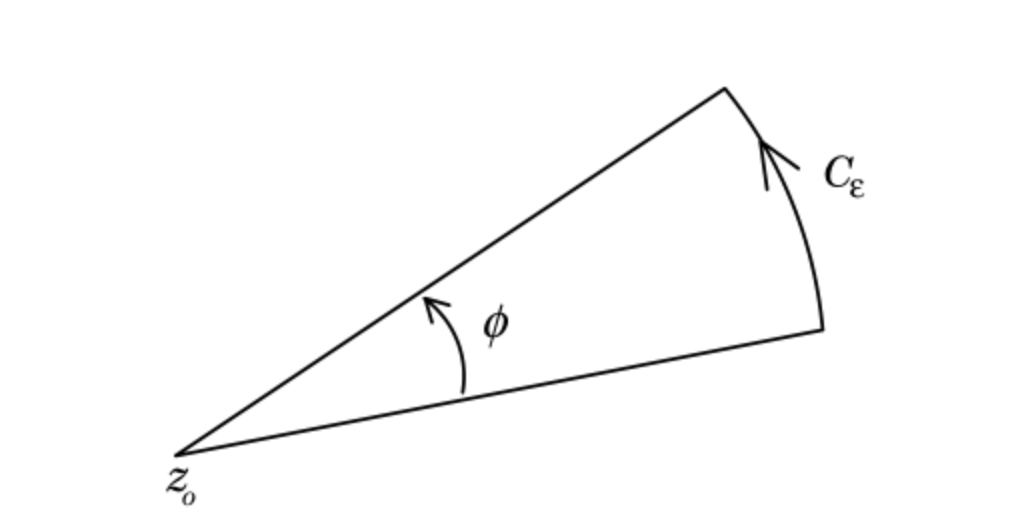
\includegraphics[scale=0.1]{./img/arc.png}
            \caption{Small circular arc $C_\epsilon$}
            \label{fig:arc}
        \end{figure}
        Using figure~\ref{fig:arc} we can rewrite~\eqref{eq:principalvalueint}
        as
        \begin{align*}
            \fint_{-\infty}^\infty f(x) \, dx &= \lim_{R\to\infty}
            \pren{\int_{-R}^a + \int_b^R} f(x) \, dx +\\
            &\lim_{\epsilon_1, \epsilon_2, \ldots, \epsilon_N \to 0^+}
            \pren{
                \int_{a}^{x_1-\epsilon_1} +
                \int_{x_1 + \epsilon_1}^{x_2-\epsilon_2} +
                \cdots +
                \int_{x_N + \epsilon_N}^{b}
            } f(x) \, dx
        \end{align*}
        A handy theorem follows.
        \begin{thm}
            \begin{easylist}[enumerate]
                @ Suppose that on the contour $C_\epsilon$ we have $(z-z_0)f(z)\to0$
                uniformly as $\epsilon\to0$. Then
                \begin{align*}
                    \lim_{\epsilon\to0} \int_{C_\epsilon} f(z) \, dz = 0
                \end{align*}
                @ Suppose $f(z)$ has a simple pole at $z=z_0$ with residue
                $\text{Res}(f(z); z_0) = C_{-1}$. Then for the contour
                $C_\epsilon$
                \begin{align*}
                    \lim_{\epsilon\to0} \int_{C_\epsilon} f(z) \, dz =
                    i \phi C_{-1}
                \end{align*}
                where the integration is carried out in the positive
                (counterclockwise) sense.
            \end{easylist}
        \end{thm}
        Basically, what we're doing here, is taking the limit as the bounds on
        the real integral go to infinity, and looping around through the complex
        plane, using the nice properties we get from the complex plane.

        \subsubsection{Integrals With Branch Points}
        We can use the same strategy to integrate functions with branch points.
        \begin{thm}
            If on a circular arc $C_R$ of radius $R$ and center $z=0$,
            $zf(z)\to0$ uniformly as $R\to\infty$, then
            \begin{align*}
                \lim_{R\to\infty} \int_{C_R} f(z) \, dz = 0
            \end{align*}
        \end{thm}

    \subsection{The Argument Principle, Rouch\'e's Theorem}
    \begin{thm}[Argument Principle]
        Let $f(z)$ be a meromorphic function defined inside and on a simple
        closed contour $C$, with no zeros or poles on $C$. Then
        \begin{align*}
            I =
            \frac{1}{2\pi i} \oint_C \frac{f^\prime(z)}{f(z)} \, dz =
            N - p =
            \frac{1}{2\pi} \bren{\arg f(z)}_C
        \end{align*}
        where $N$ and $P$ are the numbers of zeros and poles, respectively, of
        $f(z)$ inside $C$; where a multiple zero or pole is counted according to
        its multiplicity, and where $\arg f(z)$ is the argument of $f(z)$; that
        is, $f(z)=\abs{f(z)} \exp(i \arg f(z))$ and $\bren{\arg f(z)}_C$ denotes
        the change in the argument of $f(z)$ over $C$.
    \end{thm}
    The quantity $\frac{1}{2\pi i} \bren{\arg w}_{\widetilde{C}}$ is called the
    winding number of $\widetilde{C}$ about the origin. %TODO insert image on pg274
    \begin{thm}[Rouch\'e]
        Let $f(z)$ and $g(z)$ be analytic on and inside a simple closed contour
        $C$. If $\abs{f(z)} > \abs{g(z)}$ on $C$, then $f(z)$ and
        $\bren{f(z)+g(z)}$ have the same number of zeros inside the contour $C$.
    \end{thm}

    \subsection{Fourier and Laplace Transforms}
    In suitable function spaces, defined below, the Fourier transform pair is
    given by the following relations:
    \begin{align*}
        f(x) &= \frac{1}{2\pi} \int_{-\infty}^\infty \hat{F}(k) e^{ikx} \, dk\\
        F(x) &= \int_{-\infty}^\infty f(k) e^{-ikx} \, dx\\
    \end{align*}
    $\hat{F}(k)$ is called the Fourier transform of $f(x)$. The other one is
    called the inverse Fourier transform.

\section{Notes}
    \subsection{Exams}
    \begin{easylist}
        @ Exam 1
        @@ 1.1 - 2.5
        @ Exam 2
        @@ 2.6 - 3.5
        @ Exam 3
        @@ 3.3, 3.5, 4.1-4.5
    \end{easylist}

    \subsection{Trig Identities}
    \url{http://www.sosmath.com/trig/Trig5/trig5/trig5.html}
    \begin{figure}[H]
        \centering
        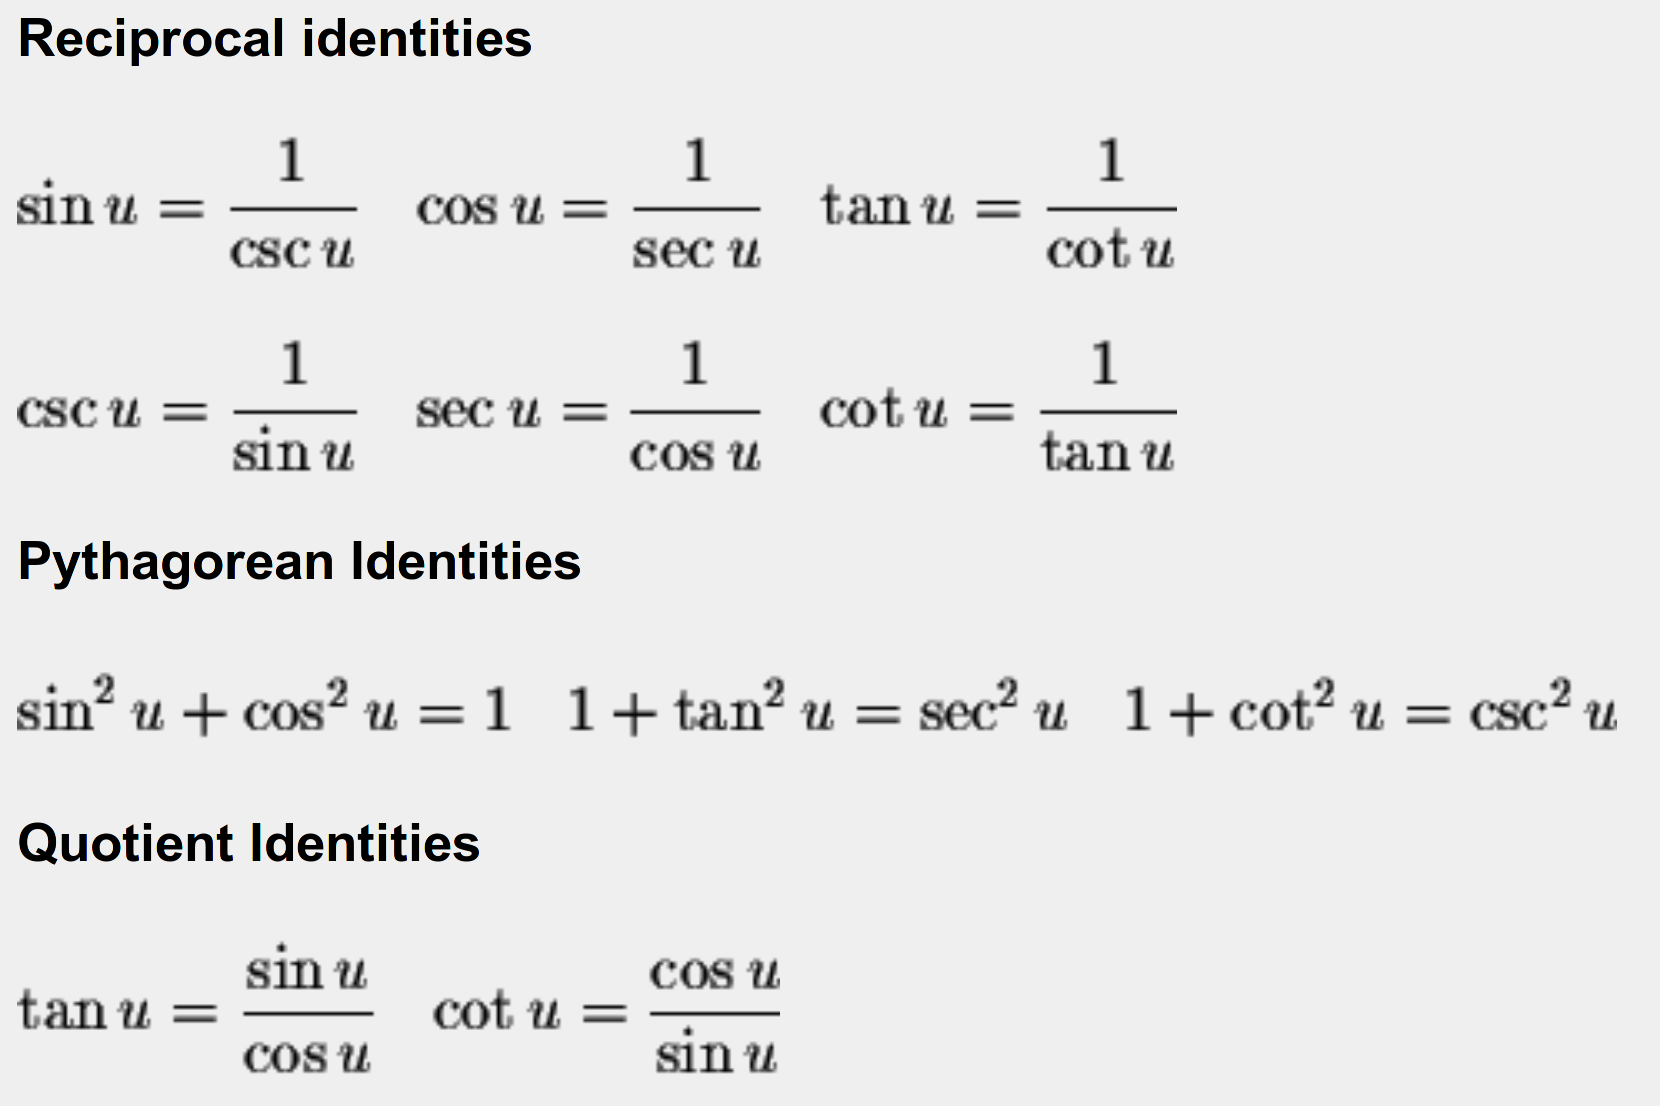
\includegraphics[scale=0.2]{img/trig0.png}
    \end{figure}
    \begin{figure}[H]
        \centering
        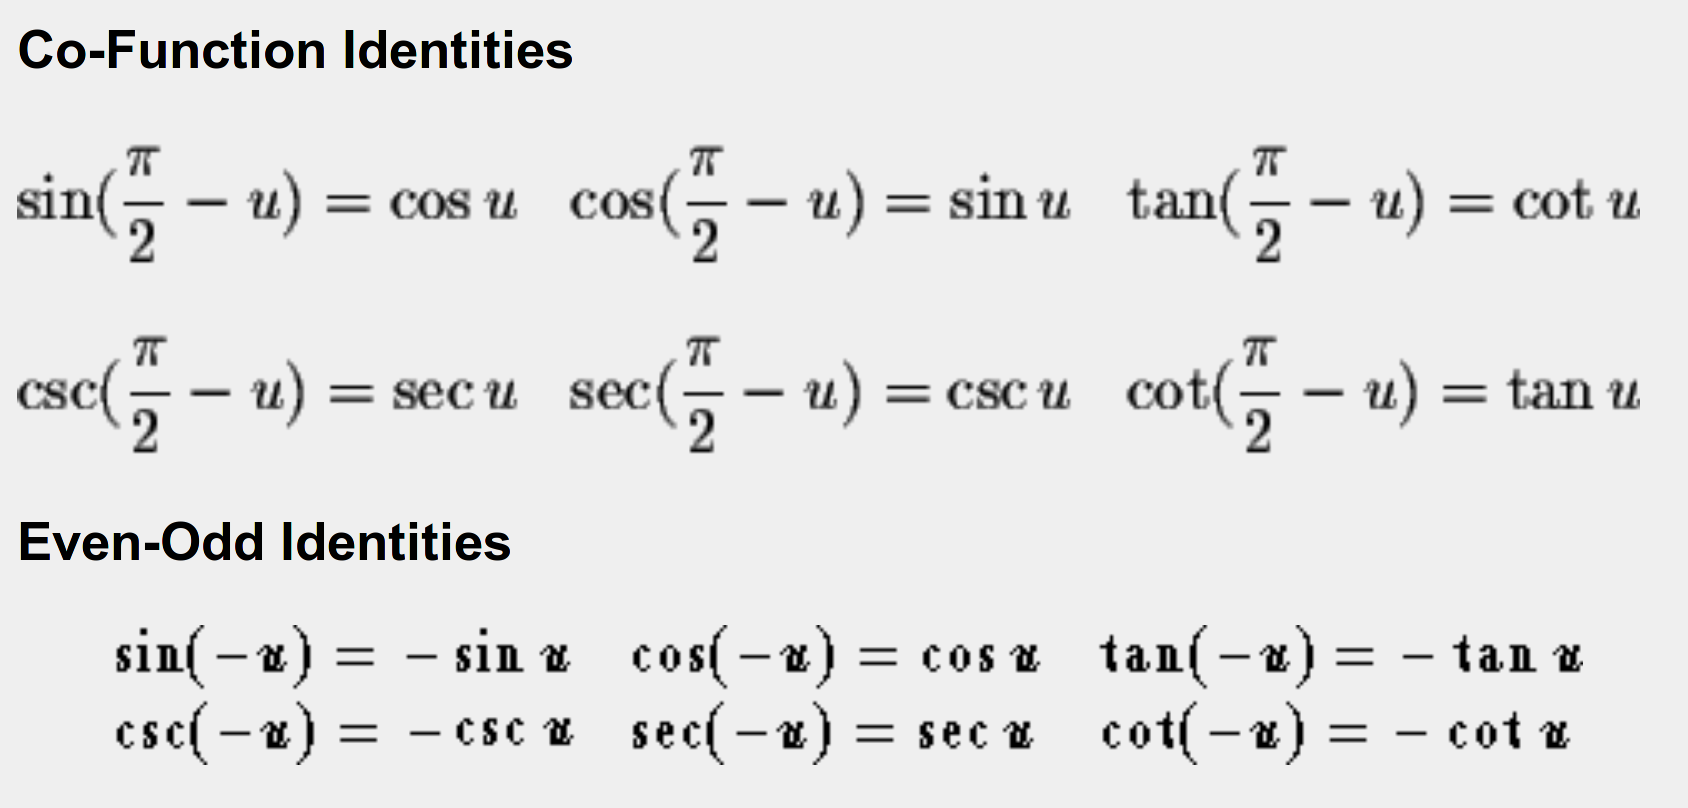
\includegraphics[scale=0.2]{img/trig1.png}
    \end{figure}
    \begin{figure}[H]
        \centering
        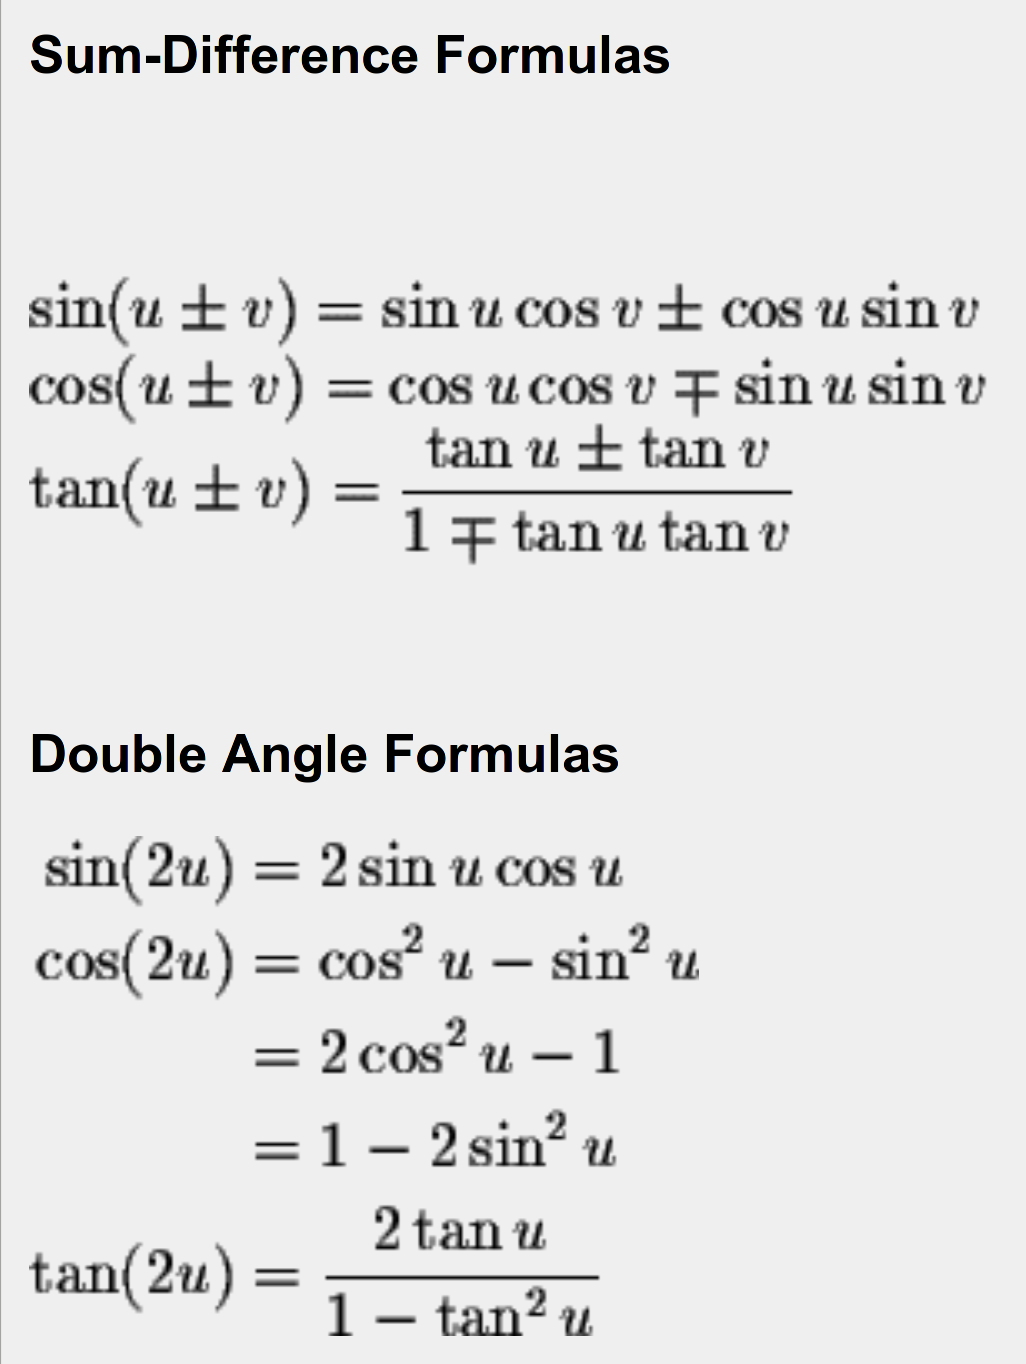
\includegraphics[scale=0.2]{img/trig2.png}
    \end{figure}
    \begin{figure}[H]
        \centering
        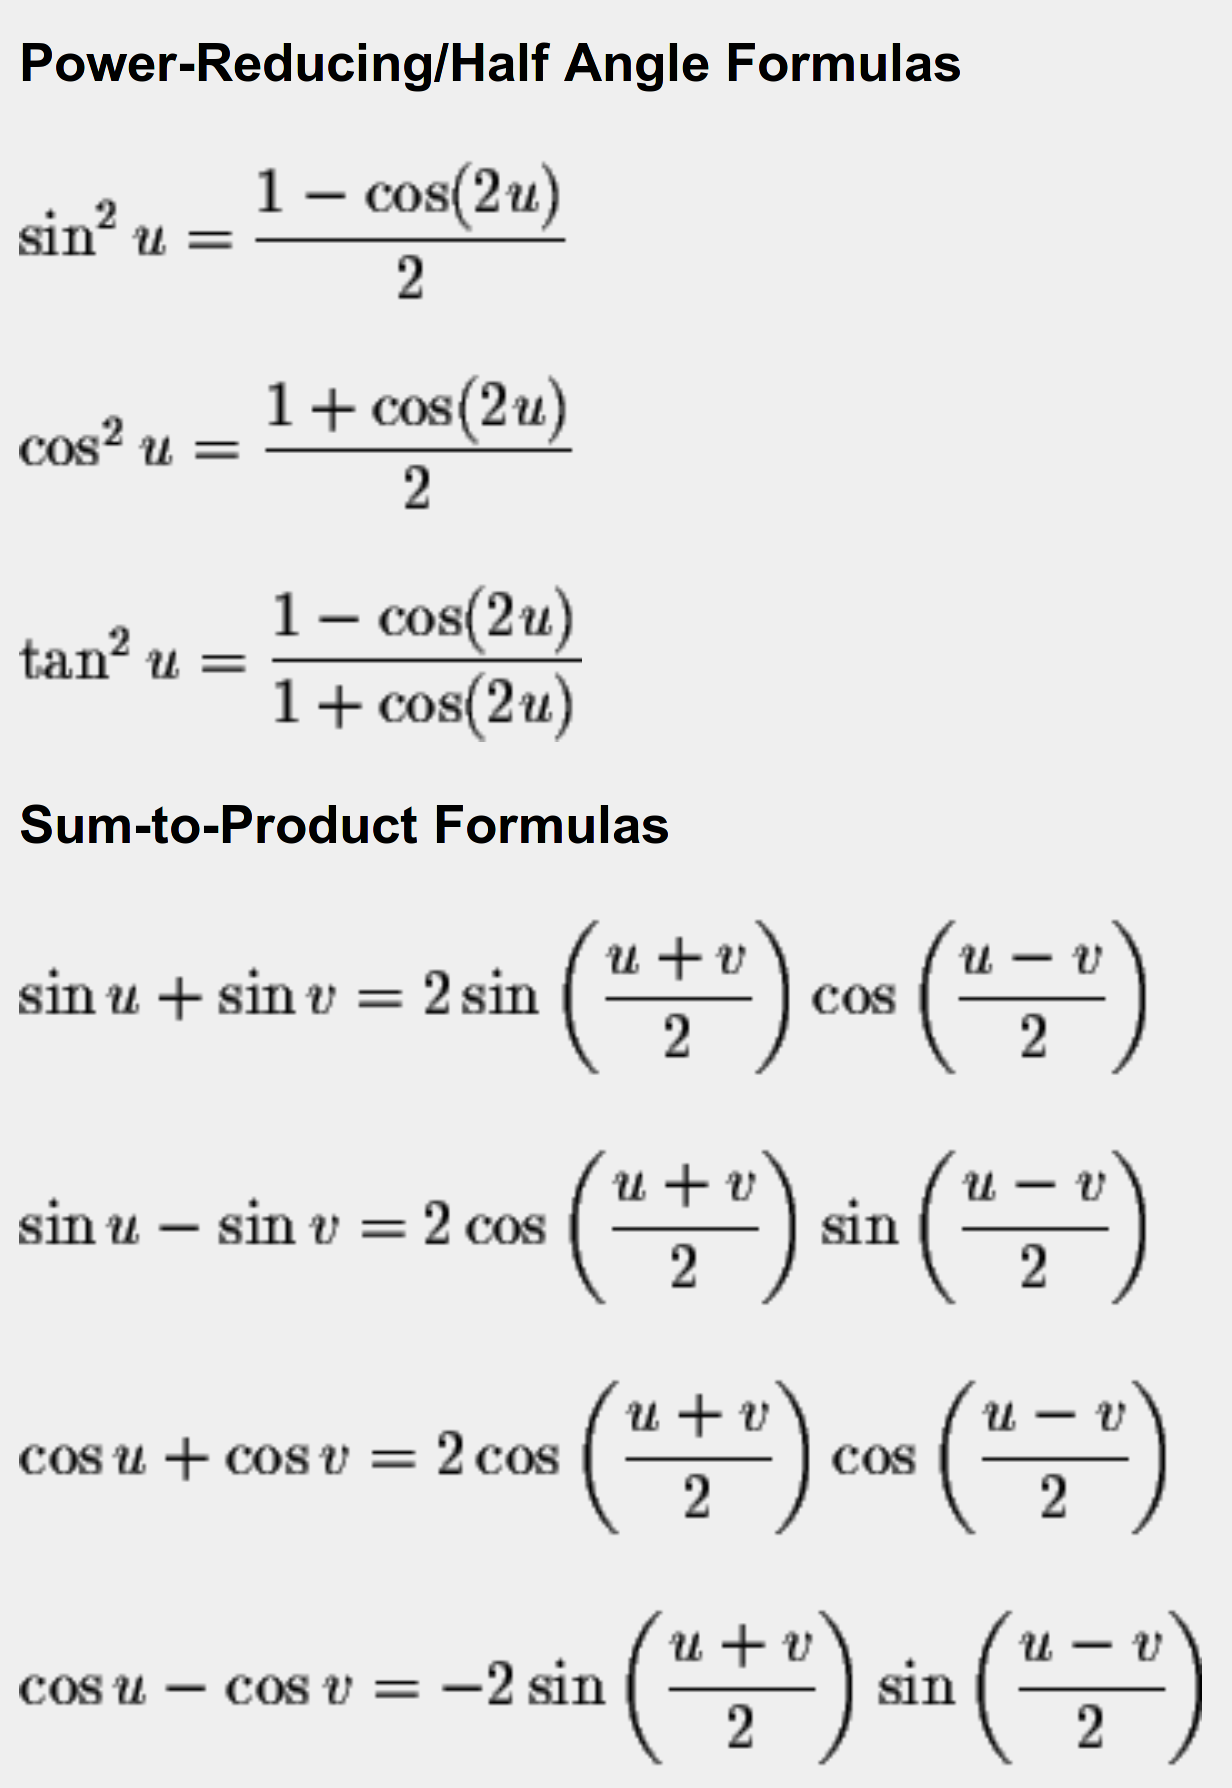
\includegraphics[scale=0.2]{img/trig3.png}
    \end{figure}
    \begin{figure}[H]
        \centering
        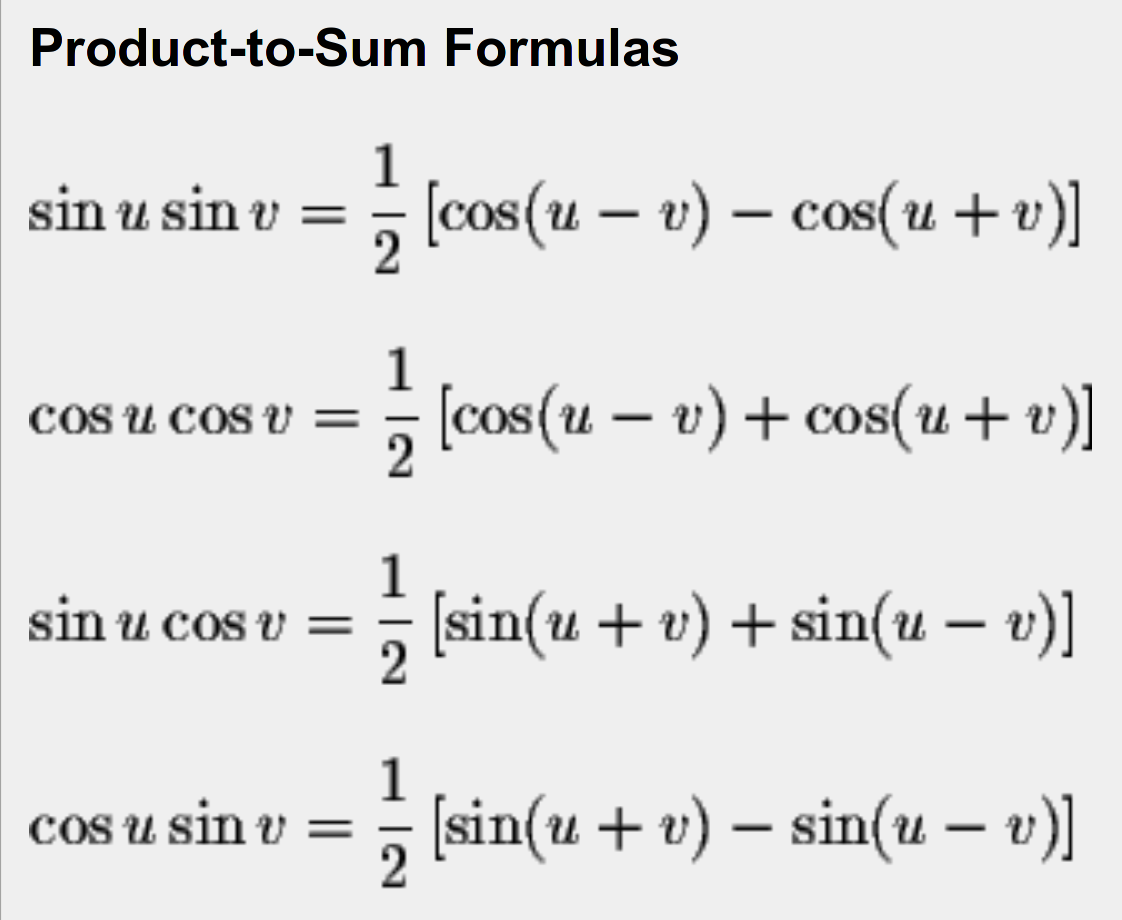
\includegraphics[scale=0.2]{img/trig4.png}
    \end{figure}
